\chapter{Student-Created OurPlace Activities}
\label{chap:student-created}

\todo[inline]{Placeholder text from paper}

\section{Overview}
Blumenfeld et al. lament that small, easily assessed tasks which focus on low-level facts and skills (i.e. tasks commonly found on worksheets) have become the focus of many classrooms \cite{Blumenfeld1991}. They argue that these tasks afford students `\textit{few opportunities to represent knowledge in a variety of ways, pose and solve real problems, or use their knowledge to create artefacts}'. Arguably this can be at least partly attributed to pressures and limitations put upon teachers and schools, as they work within structures which expect them to conform to quantifiable testing methods, propagating the aforementioned worksheet-style tasks and `teaching to the test'. The head of the UK's Office for Standards in Education (Ofsted) has noted that `\textit{[Ofsted] have created a situation where second-guessing the test can trump the pursuit of real, deep knowledge and understanding}' \cite{Ofsted2018}. Blumenfeld et al. argue that a preferable alternative is project-based learning (PBL), which they describe as an approach to teaching and learning which focuses on engaging students through the investigation of non-trivial, `authentic' problems in a manner which supports learner autonomy over the course of an extended project \cite{Blumenfeld1991}. These projects frequently involve the creation of public artefacts, employing constructionist learning processes \cite{PapertSeymourandHarel1991a, Holubova2008}. However, the restrictions placed upon teachers frequently impacts their available teaching time, curriculum content and pedagogical approaches. This has meant that implementing project-based learning in UK schools has proven to be a challenge \cite{TheEducationEndowmentFoundation2016}.

\begin{figure}
\centering
  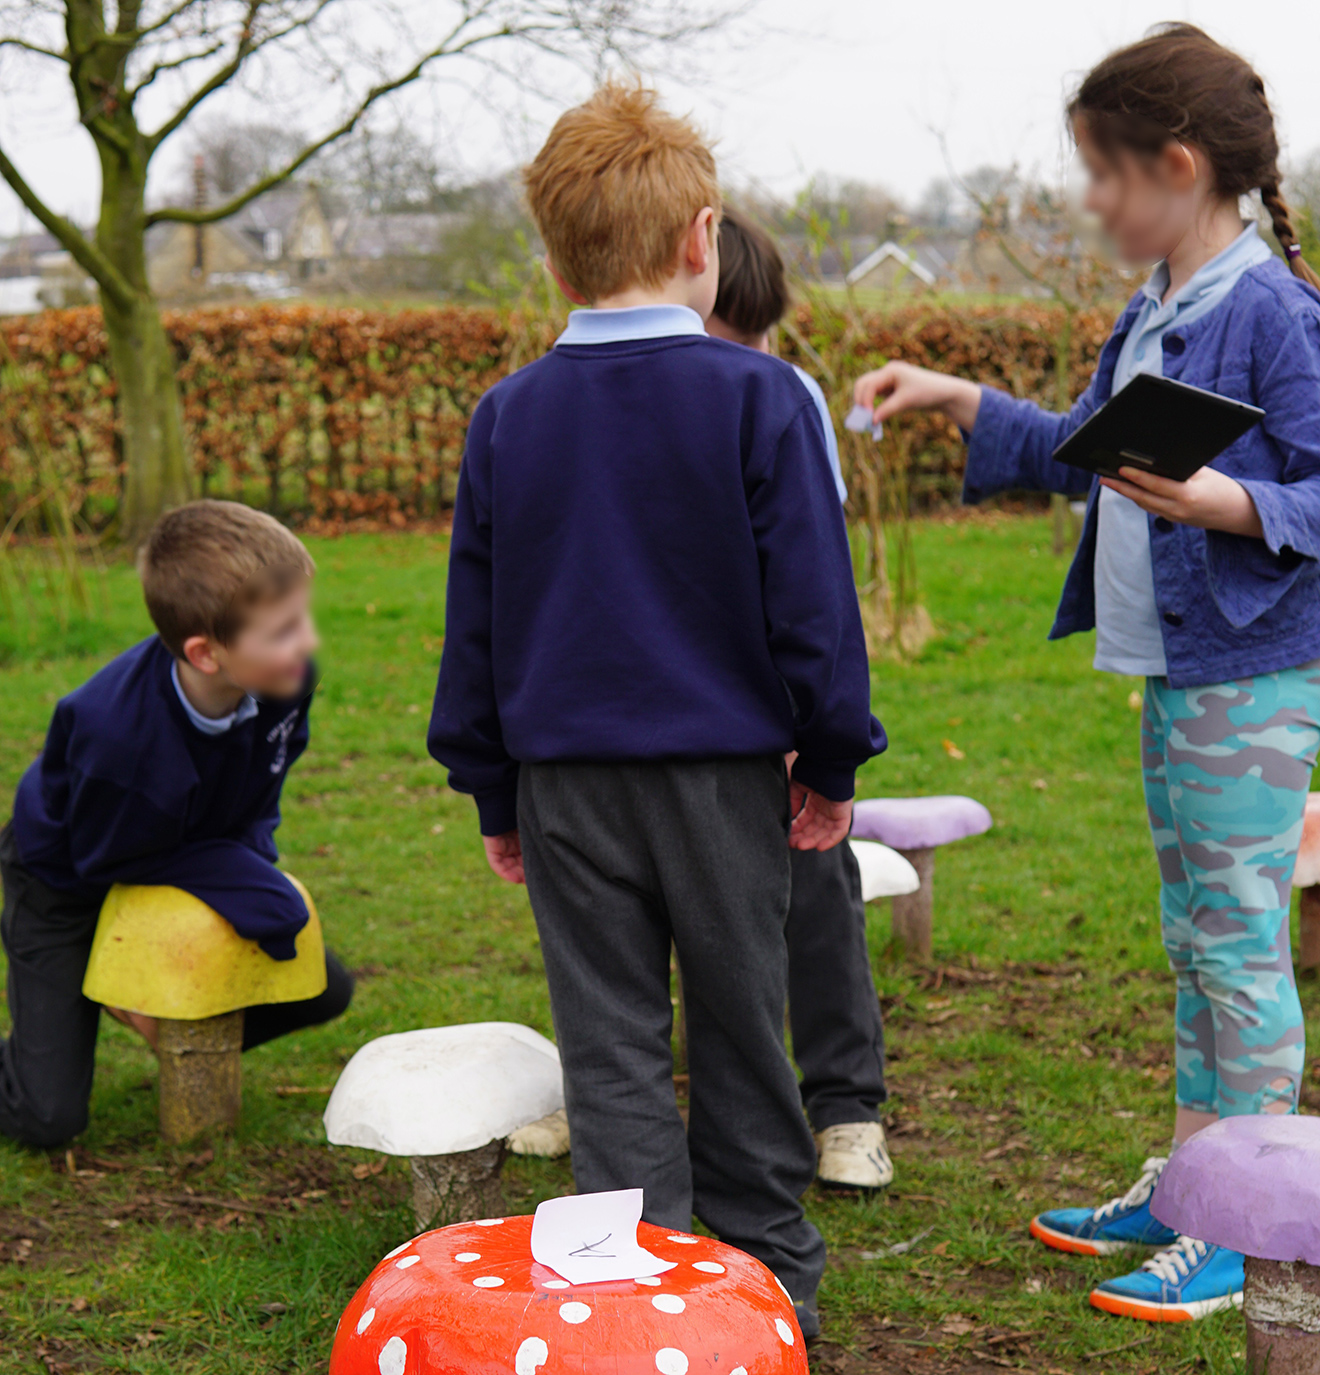
\includegraphics[width=0.66\columnwidth]{images/chapter08/mushrooms.jpg}
  \caption{A Year 4 student reveals a clue to some younger classmates, leading them to the mobile learning activity's next objective. }~\label{fig:Mushrooms}
  \vspace{-2.3em}
\end{figure}

At the same time, mobile learning (`\textit{learning across multiple contexts, through social and content interactions using personal electronic devices}' \cite{Crompton2013}, AKA `m-learning') has grown to play a large role within schools in the UK, with access to tablet computers becoming more common in schools (44\% of UK schools are expected to have one tablet per child by 2020 \cite{BritishEducationalSuppliersAssociation2015}), and their general ubiquity meaning most of the younger population is familiar with their use (84\% of UK children aged between 8--16 report owning a smartphone \cite{Statistica2018a}). Despite this, there is a lack of HCI research around how m-learning technologies can be used for artefact creation in PBL \cite{Chan2015}.

In this paper, we explore the concept of `project-based mobile learning' (PBML) through the creation of a PBML framework, and contribute insights from its application in studies held with three different UK schools and a summer school of Travelling Showmen. We contribute the framework, suggestions for its configuration in response to contextual challenges, reflections on how PBML harnessed students' existing desires for independence, and how it could offer new avenues for leveraging place as a learning resource. We conclude by arguing for further exploration of how mobile technologies can support the creation and sharing of interactive content within PBL.

\section{A Project-Based Mobile Learning Curriculum}
This project was undertaken through a design-based research approach: one in which researchers work alongside practitioners (i.e. teachers) in naturalistic settings, and produce multiple iterations of designed interventions to explore theoretical relationships \cite{Barab2004}. For these studies, we wished to explore the potential for m-learning applications to be used as constructionist tools within a PBL process, used by students to create new learning resources for use by their peers. To this end, we designed a PBML framework for use within UK schools. In this section we introduce this framework, and the OurPlace application with which we chose to apply it.

\subsection{Overview of the PBML Framework}
We knew that any PBL programme would have to be able to adapt to variations in teachers' time, teaching requirements and levels of mobile hardware access \cite{Blumenfeld1991, Krajcik2006, InnovationUnit2016, TheEducationEndowmentFoundation2016}. In response, we designed an adaptable five-stage framework based on the essential elements of PBL \cite{Larmer2015}. This framework asks students to create a mobile-learning artefact as a final public entity, following a series of PBL engagements in response to their teacher's chosen topic. The stages, and how we applied them using OurPlace, are described below.

\subsubsection{Demonstrating the Medium}
This stage gives students a hands-on example of an exemplar application of the technology, allowing them to become familiar with its potential and encouraging them to bear the technology's capabilities in mind when formulating ideas during the following stages. Demonstrating the technology on the school grounds allows students to explore its use in a safe outdoor environment, and doesn't require the overhead of additional teaching assistants. For OurPlace, students should be introduced to the structure of an Activity and be given some examples of how the different Task Types can be implemented. This could be performed with an example Activity, created to demonstrate all of the different Task Types available.

\subsubsection{Researching the Domain}
As with most other forms of PBL, a significant amount of time is allotted to students investigating the given problem domain. This is likely to be assisted in some way by technology, however other options exist such as fieldwork (e.g. site visits, performing interviews) and offline research (e.g. in libraries). A degree of autonomy should be granted to the students, however some guidance may be required.

\subsubsection{Prototyping}
In this stage, students create a low fidelity (e.g. pen and paper) prototype of their public entity, using their research as content. Our reasoning for doing this outside of the technology is that it: (i) doesn't require access to mobile hardware; (ii) lets students design without having to simultaneously learn the technology's authoring interface; (iii) emphasises the learning focus as being on the content, rather than the technology \cite{Bell2010}; and (iv) supports tangible interactions and visual learning and thus more easily supports collaboration between students \cite{Stanton2001}. Example prototypes might consist of storyboard or map-based activities.

To prototype OurPlace Activities we created a jigsaw exercise, where students can design different configurations of their Activities (Figure~\ref{fig:JigsawToApp}). The jigsaw's structure is directly analogous to that of an Activity: a single piece is dedicated to the its title, description and cover image (i.e. Figure~\ref{fig:ActivityCreation}.A), with the Activity's Tasks represented as separate pieces connecting to it and chaining together. Each Task's jigsaw piece has a slot for a smaller Task Type piece, and the jigsaw allows for Task pieces to be connected in different directions to indicate Follow-Up Tasks. Pieces feature a layer of sticky-back plastic and are written on with dry-wipe pens, allowing the students to make amendments and the jigsaws to be reused. Students' finished prototypes are photographed for later reference.

\subsubsection{Creating \& Refining}
This stage involves the creation, testing and iteration of the public entity using the m-learning technology. If the students created a prototype, this could simply serve as a digitisation process. For OurPlace, this involves creating Activities within the mobile application, and requires guidance from the educator/researcher as to how the creation process works. Once finished and uploaded, students may want to try their Activities and refine them in response to any issues they encounter. 

\section{Studies}

We needed to assess how well this curriculum would work when applied within a real school context and how it could be configured to adapt to a given school's time and resource limitations. In this section we discuss studies held with three different formal education schools in the North East of England, as well as engagements held with a summer school of Travelling Showmen. Each has their own socio-economic and cultural backgrounds alongside a unique locality.

\subsection{Research Methods \& Data Collection}

All student interactions with the OurPlace application took place through Android tablets provided by the researchers, with the tablets' Internet connectivity provided by the researchers' wireless router and SIM card. The first author was present whenever the app was in use (unless noted), providing technical support as necessary and taking field notes and audio recordings. No identifiable information on the student participants was collected with the exception of photographs, which were only taken with prior parental consent. Any names given below are pseudonyms. Semi-structured interviews were held with the teachers after the engagements, with a mixture of oral and written feedback given by students. A thematic approach to coding was performed across all of this data, with codes being qualitatively analysed by the authors before grouped into final themes.

\subsection{Configuration 1: Without Prototyping}
The first group we engaged with was a Year 8 history class (age 12-13, N=32) in a secondary school (School 1) based in a moderately affluent village. We approached the school's leadership about the possibility of them doing a PBML project: the school's headteacher agreed and assigned the class's history teacher (T1) to the study. As with many other secondary school teachers in the UK, T1 was under pressure to prepare the students for frequent formal assessments, and so was reluctant to dedicate much teaching time to the project. When we were organising the study, they noted: `\textit{Workload and time would be the main issues---the commitment it would take up in lesson time. It would be difficult to slot something additional like this in around key assessment work, and also keeping it relevant to the curriculum we are following}'. As a result, the project was given a very short amount of classroom time---only two hour-long sessions, with further work to be done by students outside of school. Observations of two of T1's other lessons suggested that they preferred an `authority' or lecture style of teaching. T1 appeared ambivalent towards PBL approaches, and when queried on their opinion of them noted `\textit{It's not the way we do things here}'.

T1 already possessed a paper-based history trail of the local village, designed for use by younger students joining the school. For the study, T1 tasked the class to use OurPlace to create digital trails in pairs, featuring historical elements of their choosing. Prior to our first session with the students, T1 provided them with a lengthy PDF document and a PowerPoint presentation, which detailed most of the historical buildings in the village, serving a starting point for researching content. Prior to the first session, T1 expected that the students should be fairly well prepared in terms of trail content: `\textit{The students should already have ideas of what they want to do, but are waiting to see what the software will do. The issue is what the software can do and whether it can easily tied in with the plans they have made already.}'  As such, the `Researching the Domain' stage took place earlier in the process than planned. T1 was also concerned about the students' work being able to function outside of an m-learning context, hoping to also have `analogue' versions of the students' trails: `\textit{Could a finished product be adapted to be used at another time even if no iPads were available---maybe some of the ideas usable in a non-digital way?}' To this end, they encouraged students to try and design their digital trails such that they would be adaptable to a pen and paper format.

T1 decided to make the majority of the Activity creation process a homework task, with students using their own devices outside of school. This was mainly in response to the extremely limited amount of classroom teaching time that could be dedicated to the project: because we also wanted to go through the students' final Activities, that only left a single hour-long session to work with the students in class. In order to prepare the students for this independent work, our first hour-long session was spent \textit{Demonstrating the Medium}. This involved the students completing an example OurPlace Activity on the school grounds, demonstrating all of the Task Types and several instances of Follow-Up Tasks. Upon returning to the classroom, the rest of the session (around 20 minutes) was spent introducing the students to OurPlace's Activity creation tools. By the end of the hour, all students reported that they understood the app, what it could do, and how to make their own Activity.

During the second session three weeks later, a researcher and T1 sat with the students and went through their Activities. While most of the pairs had produced an Activity, they tended to be quite short (averaging 4 Tasks per Activity) and shallow: most of the Activities served more as explorations of the different interactions possible with OurPlace than a meaningful engagement with the subject matter. For example, one student's Activity asked the learner to simply find and photograph an `area of interest'. Despite this, many of the students had engaged strongly with the process and had taken ownership over their Activities: for example, one student's trail featured characters they had created for their personal YouTube channel. However, as a result of the focus on technology interactions, many students struggled in fulfilling the teacher's requirement of creating a paper-based version of their Activity. One pair of students had more success, claiming `\textit{I think we've found it easier than other groups because we focused more on the content than using all of the different interactions. So a lot of the content can be the same, it's just changing how to interact with it}'. Due to teaching time limitations, the Activities were not shared between students or used outside of the classroom.

T1 noticed the students' focus on interactions with the technology over engaging more deeply with the historical content. In the follow-up interview, they noted: `\textit{The thing I was coming across again and again was the lack of challenge, the lack of depth, and the kind of things they were asking was really just playing with the technology rather than [engaging with the history]}'. This surprised T1, as they had been expecting any issues encountered to have resulted from the introduction of new technology, rather than the students' research: `\textit{I think it's more of a success for the medium than the actual content. [...] Maybe not what I expected, actually--in some ways maybe the opposite}'. T1 argued that without the deeper integration of research and knowledge into the Activities, they are of little value: `\textit{It needs to be worth doing: there's no point in having all of the bells and whistles if there's no substance}'. They noted that this could have been improved through a reconfiguration of the PBML framework to offer more structure: `\textit{It's worth cogitating about what parameters you probably need to introduce, to guide them towards deeper thinking. I know that if that had been more free-form and open-ended, that would have been rather worse}.' T1 suggested that when applying content knowledge to Activities, a balance needed to be struck between a more guided, restrictive approach and supporting students' creativity and autonomy: `\textit{If they were highly creative and lost their focus, then they'd be miles [off]. If they were less creative, but focused on the nature of the content, they'd probably find it easier to transpose. What we want is something in-between}'.

\subsection{Configuration 2: Full Process}
We worked with two different schools over an extended period of time (10-12 hours of sessions per school, spread over several weeks) to deliver a more fully-implemented version of the framework. This was partly supported by the fact that we were working with Year 4 (age 8-9) classes---as less focus is placed on preparing for examinations, we've found that pre-secondary school teachers are more willing to engage with experiential forms of learning. Both schools welcomed the implementation of a longer project over several sessions.

\subsubsection{Engagements with School 2}

The first of these schools (School 2) was based in a tiny rural village. We worked with the entirety of the Year 4 group, who were the oldest children in the school (age 8-9, N=7). Because the school's population is so small, Year 3 and Year 4 share the same classroom. The class teacher (T2) had approached us about using PBML to augment orientation and map-reading with new technologies in lessons. With a generous scope and large amount of time available, we decided that the students would do two projects: one to learn the mechanics of making Activities, and another which focused on their village's heritage. 

For the first project, we tasked the Year 4 students with individually creating OurPlace Activities for their younger classmates to complete around the school grounds. As with School 1, the first session started \textit{Demonstrating the Medium} through an example Activity. We then moved straight to the \textit{Prototyping} phase, as these first projects didn't require any research. While the students initially struggled conceptually with the jigsaws due to their abstract nature, after a few minutes they understood the links between the puzzle pieces and the structure of the app. The children all settled on creating some form of `adventure', where each Task was a riddle to solve in order to find locations within the school. Tasks included finding QR codes around the school, and finding specific locations using `Photo Match'. We found that their Activities made use of most of the different Task Types available, which may have been encouraged by the jigsaw packs having a limited quantity of each Task Type piece, forcing students to diversify (however, some students overcame this by simply not placing a Task Type piece if their chosen one wasn't available--see Figure~\ref{fig:JigsawToApp} as an example). This highlights the potential for prototyping in a physical medium to provide constraints.

In the second two-hour session the students used their jigsaws as references to assemble their OurPlace Activities (Figure~\ref{fig:JigsawToApp}). Most were happy working independently, and reported that their jigsaws made learning the creation process `\textit{much easier}'. The children enjoyed exploring what they could do with the technology's functionality: for example, one student's final \textit{Listen to Audio} Task `rewarded' the user for completing their Activity with a recording of them singing the song \textit{Celebration} by Kool \& the Gang. The second session concluded with the students testing out their Activities and making refinements (mostly involving spelling errors and reordering Tasks). 

The final two-hour session of the project was spent by the students sharing with their peers. T2 briefed the younger students, giving the Year 4s positions of seniority and highlighting their efforts: `\textit{You really need to listen to what [Year 4] have to say, because they have designed this themselves. They are your teacher, OK? Please listen, because they've worked really hard, and they're really excited about you having a go.}' The Year 4s accompanied rotations of small groups of younger students as they completed their Activities around the school, with groups being swapped to allow all students to try each Activity. The Year 4s were given the responsibility of showing the younger students how the app worked, and assisting them if they got stuck (Figure~\ref{fig:Mushrooms}). The younger students were very enthusiastic, and were keen on making sure they completed each of the Year 4s' Activities. At the end of the session the Year 4s hosted a school assembly, in which they showed the other children their jigsaws and shared what they most enjoyed (`\textit{I enjoyed being the teacher'; `Being outside'; `I enjoyed making the Activity itself}') and the younger children gave them feedback (\textit{`Our favourite was [Susan's], because we got to find lots of things'; `I really liked the beeping one, the Location Hunt'}). The school's headteacher praised the Year 4s' independent work as showing maturity: `\textit{We can trust you to do something away from the class teacher and still do something really good. I think you really are stepping up to be Year 4s, it's wonderful to see. [...] If you're very grown up, you get to do very grown up things. So let's give Year 4 a clap}'. T2 also praised their leadership (`\textit{I would like to also point out how good they were as teachers, as well. They really came into their own. I was very proud of them.}') and noted that OurPlace supported a varied output: `\textit{They were very different as well weren't they? The ideas. Even though you all started off with the same tools.'}

\begin{figure}
\centering
  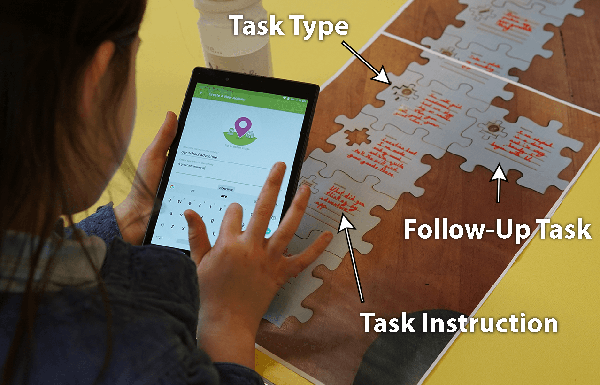
\includegraphics[width=0.7\columnwidth]{images/chapter08/jigsawToApp}
  \caption{A student uses a photograph of her jigsaw prototype as a reference for creating an OurPlace Activity. When she ran out of \textit{Location Hunt} pieces, she simply wrote the Task Type on the Task piece.}~\label{fig:JigsawToApp}
\end{figure}

Following the success of the first project, T2 was excited to start the second one. Prior to it starting, T2 preemptively collected a number of historical resources relating to the area, including newspaper articles, photographs and a book detailing the village's buildings. As T2 claimed to not have much prior local historical knowledge, this also served as their introduction to the village's heritage. T2 proceeded to make a shortlist of the more interesting buildings (such as an old blacksmith, a pub and a post office), shared these with the Year 4 students, and then took them on a short walking trip around the village so that all of the children had first-hand experience with the sites. Each child chose a different location to base an Activity on, using the walk and the teacher's resources to research it.

As the group was already familiar with the app, we skipped the \textit{Demonstrating the Medium} stage. When we asked the students if they would find it helpful to plan their Activities out using the jigsaws, they said no: they'd rather jump straight into making them using OurPlace, as they were already comfortable creating and editing using the app's tools. The Activities were produced over three hours between two sessions. All of the children's Activities featured `Location Hunt' Tasks guiding the learner to their chosen location, with further details delivered through `Information' and `Listen to Audio' Tasks. Less passive Tasks included asking the learner to draw details from the location, and a `Multiple Choice' quiz based off given information. The students then shared their Activities with the younger students in three groups, with each group accompanied by an adult and sharing tablets one-between-two. The groups completed each of the 7 Activities around the village before returning back to the school. T2 was pleased with the Activities, as the students `\textit{were able to engage with the local history in a way which they enjoyed, and they've taken pride in sharing their work with the Year 3s.}' After the trip, several of the younger students asked if they could make their own Activities the following year.

\subsubsection{Engagements with School 3}
We approached another Year 4 teacher (T3) at an inner-city school (School 3), after their class had shown an interest in local history by successfully campaigning for the installation of a commemorative plaque celebrating a notable slavery abolitionist who had lived near their school. This was particularly relevant to School 3, as it serves a large number of families of Nigerian descent. T3 was enthusiastic about the concept of producing Activities relating the the area's numerous other plaques. We worked with the majority of the school's Year 4 (age 8--9, N=21, led by T3) and Year 6 (age 10--11, N=32, led by Teacher 4) students, who worked together on the project in 14 mixed groups of 3-4.

As with School 1 and School 2, the students used a demonstration Activity as an introduction to OurPlace. Following this, T3 explained that each group was to choose and research one of the historical figures commemorated by the plaques in the area, and produce an Activity related to them. Over the following week, the teachers dedicated several hours of class time to researching and visiting the plaques. As a result, by the second engagement each group had prepared several pages of notes relating to their chosen plaque and were ready to start designing their Activities.

The School 3 children found it helpful to have a tablet for reference while constructing their prototypes, and frequently referred to their notes while writing their Tasks. The completed jigsaws were photographed and used as references for creating the Activities in a third session later that week. Part of this third session was also spent visiting the plaques with the students, so that they could test and refine their Activities and take photographs to include in them. The final session of the project involved the students going out and completing each other's Activities. Examples of the final Tasks include asking learners to `Record Video' of interviews where students role-play as their plaque's person of interest, and Follow-Up Tasks quizzing learners about the contents of `Listen to Audio' narrations. Some Activities lacked content, which T3 attributed to a lack of available information for the chosen plaque's subject and some children's behavioural issues.

When asked what their favourite part of the project was, several of the students mentioned that they particularly enjoyed sharing Activities: `\textit{[I most enjoyed] today, getting to go around and swap with other people and getting to find out about theirs}.' They also felt that swapping Activities was an important part of the process, as it could also share different ways in which the Task Types could be used. Furthermore, one Year 6 student noted that OurPlace could be used to share the value of place with visitors and other communities: `\textit{I think that if we made stuff for another school that made them learn, it would be really good because you could make it about your school.}' Teacher 4 expanded on this concept: `\textit{That would be an interesting thing to do, wouldn't it? To swap it and see what their daily life is like and what yours is like.}' 

During a follow-up interview, T3 reported to particularly like tactile nature of the jigsaw prototype: `\textit{Doing it on a piece of paper is very boring, so to get them to understand that the order can matter... I think that's a very good, visual way of showing the children. That really worked.}' Unlike the children in School 2, T3 also saw value in doing the prototyping for making further Activities: `\textit{I would use the jigsaws every time. Because it's a different Activity.}' T3 saw the jigsaws as Activity prototypes, rather than simply a way of easing the students into the application's structure. Following the study T3 requested a digital version, so that they could print copies for students to prepare future OurPlace Activities. T3 also saw a potential value in exchanging with separate groups of students: `\textit{I think it would have been better if we'd done it, and then taken a different group of children out to use it. So you do it with one class, then take the other class with them to show it. And then they can evaluate by watching the other child. But it's just time pressure, isn't it?}'

T3 was also highly favourable of teaching in authentic contexts and using the children's existing relationships with place: `\textit{It was all about taking a context specific approach, that's what I'm really into. These children know about their local area, and that helped us scaffold the Activities.}' T3 also noted that many of the children were not aware of the area's history, and that the historical figures could act as inspirational role models: `\textit{This is where the children live, so it's really important that they understand the history of it. Really great people who're like them have lived in this area.}' Furthermore, working in these environments brought the children in contact with community stakeholders: `\textit{They got to meet people when they went out and about. They met the guy who's raising money for the sculpture in the middle of the park.}' T3 also argued that using constructionist m-learning in a PBL approach helped leverage these civic resources in lessons, as the creation of public entities acted as a motivating factor: `\textit{It was how we were going to bring those [resources] into our lesson. I think that OurPlace really helped: it gave us a focus to do the history through the app, rather than just go and collect the information and then--what do we do with it?}' 

\subsection{Configuration 3: Without Demonstrating the Medium}
Through discussions with them, we discovered that T3 leads a summer school for children of families who run the local annual funfair. Following our engagements with School 3, we were invited to run a short engagement with a group of children (age 6-9, N=16) attending the summer school. These were the children of Travelling Showmen and Showomen, members of the Showmen's Guild: a trade association made up of traditionally insular cultural groups of families, who travel around the UK to run funfairs and circuses. While the children of these families (Showchildren) are registered with traditional schools, the families travel so frequently (one family claimed to work 40 events a year) that their schools send out packs of educational materials for the children to work on remotely. T3 derided these worksheet-based packs as uninteresting: `\textit{[The school packs] are super boring and often rubbish. Some schools are alright, but it's still working from a piece of paper.}' Inspired by Teacher 4's suggestion that OurPlace could be used as a medium through which daily life experiences could be shared, T3 suggested that we do a short project at the summer school: `\textit{Their lives are so different, it would actually be a nice tool to share with other children what it's like to be a Showman.}' We arranged a trip for the Year 4 class from School 3 to visit the fair, where the Showchildren would introduce them to their ways of life. The Showchildren would create OurPlace Activities, with which Year 4 could also collect data for later classroom use.

As the summer school only ran for two weeks, we only had one three-hour session in the summer school in which to introduce the Showchildren to OurPlace and have them create Activities. Following the issues found in the configuration used in School 1, we decided to try another, skipping \textit{Demonstrating the Medium} and relying on verbal instruction during the \textit{Prototyping} stage as an introduction to the app's functionality. The Showchildren were able to complete the jigsaw activity without first needing to use the application, and they gravitated towards making Activities which focused on their families' rides and stalls within the fair (e.g. Information Tasks about their families, Video and Photo Tasks capturing the rides in action). Transitioning from the jigsaw prototypes to the digital versions went similarly to the previous engagements, suggesting that the jigsaw serves as an intuitive metaphor for the application. Due to time limitations, the Showchildren were unable to test and refine their Activities.

We then ran a session in School 3, to introduce Year 4 to the concept of Travelling Showmen. The class's discussions largely centred on the concept of the Showchildren working in the fair, an idea which appeal to them: one child noted they wanted `\textit{to get money to support my family}'. However, there was a concern that as children, they wouldn't be treated as equals by adults: `\textit{you might not get paid as much, because people could want to only go to adults and think that children are not responsible yet}'. The children found the idea of inherited careers generally unappealing (most Showmen families have an occupational lineage of several generations), saying `\textit{I don't want to do my parents' job}', and `\textit{it's natural to want to do something different, [...] if you just carried on a tradition you might not really like it.}' To encourage fruitful conversation between the two groups of children, we also asked Year 4 to prepare some questions to ask the Showchildren. Many of the questions revolved around the Showchildren's independence and influence in the community (e.g. `\textit{Have you ever designed a ride?}'), their work-life balance (`\textit{Would you like shorter or longer shifts?}') and their earnings (`\textit{How much money do you earn?}'). Comparatively few of the questions focused on social aspects of the Showmen community (e.g. `\textit{Do you have any relatives who are in a different part of the world?}').

The trip occurred the following week. An education specialist from the Showmen's Guild gave a short talk to the children regarding Showman ways of life, and their experiences growing up within the community. Following this, the Showchildren and Year 4s were put into mixed groups of 4--5. Each group were given two tablets with the Showchildren's Activities, and the Showchildren were asked to guide the visitors around the fair. The Year 4s also used the Showchildren's Activities for their data collection, using the app to catalogue photos of the different rides and using \textit{Record Audio} and \textit{Record Video} Tasks to capture the Showchildren's responses to their prepared questions. Most of the questions had shifted to being about the lived experience of the Showchildren (`\textit{In a year how many places do you think you travel to?}', `\textit{Do you get to make many friends outside of the fair?}'). The Showchildren also responded with some questions of their own, querying the Year 4s' experiences with the funfair.

One of the Showchildren was particularly excited for the students to complete a `Scan the QR Code' Task, which asked them to find the child's parents' ride. However, when it was scanned they were disappointed to find that it didn't unlock any content, as there were no Follow-Up Tasks set. When this was explained, they didn't know what Follow-Up Tasks were: `\textit{What did you mean by follow-up? How do you put something in it?}' While disappointed, the child expressed interest in downloading OurPlace to make Activities at home.

\section{Discussion}
These studies have shown that configuring the PBML framework differently can meaningfully impact students' engagement with and knowledge of the domain and technology.

\subsection{Configuration and Compromise}
In these studies it was necessary to adapt our proposed framework in response to each teaching context's limitations. For example, T1 was severely limited in how much time they could dedicate due to obligations to follow a strict curriculum, and the Showmen's summer school was only running as long as the funfair was in town. It was only when working with the younger classes in Schools 2 and 3 that more time could be afforded. This was certainly not ideal for PBL-style engagements, which should engage students over the course of an extended period of time \cite{Blumenfeld1991}. Nevertheless, we argue that teaching contexts are rarely ideal, and so approaches to working within them should be adaptable and open to compromise. We wanted to explore this by implementing the framework in various real contexts which necessitated its adaptation.

We believe that skipping the prototyping stage in School 1 contributed towards the lack of engagement with the domain and put the students' main focus on the technology itself. Before taking the project away as homework, the last engagement the students had with the project was the technology's demonstration, meaning it was likely to take centre-stage in their minds. Our observations at Schools 2 and 3 suggest that inclusion of the prototyping jigsaw exercise may have brought the School 1 students' focus back to the domain's content.

The studies also highlighted the value of students sharing their creations with their classmates and/or the wider community. Students from Schools 2 and 3 emphasized the exchanging of Activities as being a particular highlight of their experiences, with students keen to both see what their peers had produced and also show off their own creations. T3 noted that had time allowed, they would have extended this sharing stage to support peer feedback between classes and groups. For the School 1 students, the lack of emphasis on sharing the created Activities with their peers or outside communities may have also reduced their value as constructionist public entities \cite{PapertSeymourandHarel1991a}.

In response to these findings, our other time-limited engagement with the Showmen's summer school used a different configuration which skipped \textit{Demonstrating the Medium}, instead focusing on the \textit{Prototyping} stage. While the jigsaws seemed to provide a somewhat serviceable introduction to the app due to the closeness of its metaphor, the full capabilities of the technology had evidently not been made clear to the Showchildren. In the case of the Showchild with the QR code, this resulted in a degree of frustration and disappointment that their Activity wasn't as fully featured as it could have been. It's unsurprising that more advanced functionality, such as Follow-Up Tasks, would be unclear to children without first demonstrating them in an example Activity.

Each configuration held its own compromises, resulting in an interesting balancing act between four elements: classroom time; supporting the learners' understanding of the technology (omission of the \textit{Demonstrating the Medium} stage led to not using the its full potential); supporting the meaningful application of content knowledge to that medium (omission of the \textit{Prototyping} stage led to shallow public entities which focused on the technology rather than the content); and enabling learners to exchange their creations, knowledge and feedback within authentic learning environments (omission of the \textit{Sharing} stage reduced the value of the entity creation process). Each of these elements was shown to be important, and compromising on any of them while still producing successful PBML engagements was difficult. However, successive projects can mitigate this by omitting certain stages as the learners become more experienced. This was shown in the second set of Activities made at School 2, where the students opted to skip the \textit{Demonstrating the Medium} and \textit{Prototyping} stages. Even this was up to some degree of teaching interpretation, as T3 noted they would use the jigsaw prototypes each time their class made new Activities. Further workarounds and compromises could also be explored: for example, T1 opted to make the \textit{Creating \& Refining} stage a homework activity, saving on classroom time. However, this raises issues around remote support and ensuring equal access to technology resources (potentially highlighting economic disparity between students).

We suggest that researchers and practitioners should weigh-up these compromises when configuring the framework according to their own motivations. For example, if full utilisation of the technology's potential isn't a priority, then the impacts of omitting \textit{Demonstrating the Medium} become less of a concern. Likewise, skipping the \textit{Prototyping} stage might be acceptable if the use of the technology is one of the main learning goals. However, we argue that omitting the other stages should be avoided as they are either key to the PBML process (research, creation) or major motivating factors (sharing public entities).

\subsection{Harnessing Students' Desire for Independence}
In these studies, many of the students we engaged with had a great desire for independence and to be respected as individuals. This was particularly evident in the School 3 class's fascination with the Showchildren's contributions to their family businesses, their lamentation at their lack of perceived responsibility when compared to adults and a desire to walk their own path rather than simply emulate their parents.

The PBML process capitalised on this quality, granting the students greater control and autonomy over their work \cite{Noss2017, Wurdinger2007}, and enabling them to approach creating Activities with greater degrees of personal input \cite{Richardson2017}. This could be seen in some of the personal touches put into their Activities, such as the Year 4's rendition of \textit{Celebration}, or the Year 8's usage of their YouTube characters. These flourishes--alongside the uniqueness of each Activity--suggest that OurPlace conforms to Noss and Hoyles' requirement that constructionist tools should be expressive enough to support exploration and ownership through construction \cite{Noss2017}. This also echoes previous research held with its predecessor, ParkLearn, in which students' sense of ownership of their responses to others' Activities was an important contributing factor towards their enthusiasm, thanks to greater degrees of freedom and independence \cite{Richardson2018}. Furthermore, the students' investment in their projects supports arguments that the greater autonomy afforded by PBL, as well as tapping into students' fluency with technology, can result in indicators of greater student engagement \cite{Wurdinger2007, Bell2010}.

When sharing their Activities with their peers, the students were clearly proud of their creations and enjoyed taking a `teaching role': they took care to guide the other students through the Activities to avoid them getting stuck without being overbearing (shown in School 2, e.g. Figure~\ref{fig:Mushrooms}). The School 2 teachers rewarded the students' performance by playing to their desire for perceived maturity, noting their growing trust in the children to perform independently and recognising their seniority amongst the students. This feedback also served as qualities for the younger students to aspire towards--some of the younger students later enquired about making their own Activities when they're older. This move to reposition the Year 4 students from a `consumer' role to one of mentorship--in which they have a degree of authorship over teaching materials--mirrors the study by Massey et al, in which they re-framed students from end-users to software developers and decision makers \cite{Massey2006}. In both cases, the learners were empowered through the creation of public entities to be able to take an active decision-making role in how technology could be used within their learning environment. The addition of the sharing stages took this a step further, granting the students the gratification of seeing others enjoy their creations.
 
We suggest that future m-learning designs can harness student's desires for independence as a motivational force by granting them opportunities for autonomy and personal flourishes, as well as platforms through which to share these personal creations. Within these studies, this was achieved through a combination of technology, configuration and context: OurPlace elevated students from consumers to producers by granting them creative control, and the creation and sharing of public entities in authentic contexts at the culmination of a PBML process bolstered their self-worth and empowered them through positions of mentorship. However, it's also worth noting this approach may not be conducive to success in all contexts, as teaching styles and cultures within different schools may be at odds with it or require re-balancing. For example, T1 was in favour of greater scaffolding, and believed that further student autonomy would be detrimental. 


\subsection{Leveraging Place through PBML}
Project-based m-learning offered new ways and motivations for the schools to engage with their area's local heritage and community, surfacing `new' educational resources which had previously gone underused. For example, T2 reported to previously know very little of the village's local history, and School 3 hadn't previously made use of the commemorative plaques as learning resources. T3 argued that using OurPlace to create the public entities gave lessons a focus and motivation needed in engaging teaching sessions, as simply collecting information would have felt aimless. T3 was also ardently in favour of the students learning more about their local context, as the historical figures within the area could serve as inspirational role models. Finally, in the Showmen study, a (compressed) PBML process also supported exposure to and greater understanding of another community's heritage. The students' preconceptions regarding the Showchildren were corrected following technology-mediated personal interactions with the community, and their topics of interest shifted from the practical to the lived experience of being a Showman.

We argue that PBML is particularly well suited to leveraging these local resources, as it combines the advantages of constructionism and project-based learning (supporting the ownership and exploration of ideas through the construction of public entities, in a process which encourages student inquiry and autonomy \cite{Noss2017, Larmer2015}) and those of situated, outdoor learning (experiential learning, embedded in authentic contexts \cite{Lave1991}). M-learning technologies are uniquely suited to assist this process, due to their ability to leverage these authentic physical and social learning resources and support greater degrees of student control, communication and creativity seamlessly across different learning environments \cite{Sharples2007, Richardson2018}. As noted by Chan et al., the use of mobile technologies in project-based learning has been under-researched \cite{Chan2015}. Given these apparent advantages, we would like to see future research explore how PBML could benefit from other technologies which support the creation and sharing of interactive content, rather than simple knowledge consumption or the creation of passive artefacts (e.g. blogs).

\section{Conclusion}
We have reported on and discussed four studies exploring different configurations of a project-based, m-learning framework in distinct learning contexts. A limitation of this research is that they were only loosely tied into each school curriculum, and didn't assess learning outcomes. We hope that future engagements can offer deeper integration into existing curricula and feature formal assessments, supporting further insights into how PBML can fit into wider school systems. We gained an appreciation of the importance of understanding each learning context, and how configuring the use of technologies to fit the particular demands of a context can result in effects which compromise the learning experience. We also discussed how the PBML process can harness students' existing desires for independence as a motivational force by granting them opportunities for autonomy, creativity and personal flourishes. Finally, we discussed how PBML offered new avenues for schools to leverage their local heritage as learning resources, and argue that the potential roles for m-learning technologies within project-based learning processes should be further explored.
